%Style
\documentclass[12pt]{article}
\usepackage[top=1in, bottom=1in, left=1in, right=1in]{geometry}
\parindent 22pt
\usepackage{fancyhdr}

%Packages
\usepackage{adjustbox}
\usepackage{amsmath}
\usepackage{amsfonts}
\usepackage{amssymb}
\usepackage{bm}
\usepackage[table]{xcolor}
\usepackage{tabu}
\usepackage{makecell}
\usepackage{longtable}
\usepackage{multirow}
\usepackage[normalem]{ulem}
\usepackage{etoolbox}
\usepackage{graphicx}
\usepackage{tabularx}
\usepackage{ragged2e}
\usepackage{booktabs}
\usepackage{caption}
\usepackage{fixltx2e}
\usepackage[para, flushleft]{threeparttablex}
\usepackage[capposition=top]{floatrow}
\usepackage{subcaption}
\usepackage{pdfpages}
\usepackage{pdflscape}
\usepackage{natbib}
\usepackage{bibunits}
\definecolor{maroon}{HTML}{990012}
\usepackage[colorlinks=true,linkcolor=maroon,citecolor=maroon,urlcolor=maroon,anchorcolor=maroon]{hyperref}
\usepackage{marvosym}
\usepackage{makeidx}
\usepackage{tikz}
\usetikzlibrary{shapes}
\usepackage{setspace}
\usepackage{enumerate}
\usepackage{rotating}
\usepackage{epstopdf}
\usepackage[titletoc]{appendix}
\usepackage{framed}
\usepackage{comment}
\usepackage{xr}
\usepackage{titlesec}
\usepackage{footnote}
\usepackage{longtable}
\newlength{\tablewidth}
\setlength{\tablewidth}{9.3in}
\setcounter{secnumdepth}{4}

\titleformat{\paragraph}
{\normalfont\normalsize\bfseries}{\theparagraph}{1em}{}
\titlespacing*{\paragraph}
{0pt}{3.25ex plus 1ex minus .2ex}{1.5ex plus .2ex}
\makeatletter
\pretocmd\start@align
{%
  \let\everycr\CT@everycr
  \CT@start
}{}{}
\apptocmd{\endalign}{\CT@end}{}{}
\makeatother
%Watermark
\usepackage[printwatermark]{xwatermark}
\usepackage{lipsum}
\definecolor{lightgray}{RGB}{220,220,220}
%\newwatermark[allpages,color=lightgray,angle=45,scale=3,xpos=0,ypos=0]{Preliminary Draft}

%Further subsection level
\usepackage{titlesec}
\setcounter{secnumdepth}{4}
\titleformat{\paragraph}
{\normalfont\normalsize\bfseries}{\theparagraph}{1em}{}
\titlespacing*{\paragraph}
{0pt}{3.25ex plus 1ex minus .2ex}{1.5ex plus .2ex}

\setcounter{secnumdepth}{5}
\titleformat{\subparagraph}
{\normalfont\normalsize\bfseries}{\thesubparagraph}{1em}{}
\titlespacing*{\subparagraph}
{0pt}{3.25ex plus 1ex minus .2ex}{1.5ex plus .2ex}

%Functions
\DeclareMathOperator{\cov}{Cov}
\DeclareMathOperator{\var}{Var}
\DeclareMathOperator{\plim}{plim}
\DeclareMathOperator*{\argmin}{arg\,min}
\DeclareMathOperator*{\argmax}{arg\,max}

%Math Environments
\newtheorem{theorem}{Theorem}[section]
\newtheorem{claim}[theorem]{Claim}
\newtheorem{assumption}[theorem]{Assumption}
\newtheorem{definition}[theorem]{Definition}
\newtheorem{hypothesis}[theorem]{Hypothesis}
\newtheorem{property}[theorem]{Property}
\newtheorem{example}[theorem]{Example}
\newtheorem{condition}[theorem]{Condition}
\newtheorem{result}[theorem]{Result}
\newenvironment{proof}{\paragraph{Proof:}}{\hfill$\square$}

%Commands
\newcommand\independent{\protect\mathpalette{\protect\independenT}{\perp}}
\def\independenT#1#2{\mathrel{\rlap{$#1#2$}\mkern2mu{#1#2}}}
\newcommand{\overbar}[1]{\mkern 1.5mu\overline{\mkern-1.5mu#1\mkern-1.5mu}\mkern 1.5mu}
\newcommand{\equald}{\ensuremath{\overset{d}{=}}}
\captionsetup[table]{skip=10pt}
%\makeindex


\newcolumntype{L}[1]{>{\raggedright\let\newline\\\arraybackslash\hspace{0pt}}m{#1}}
\newcolumntype{C}[1]{>{\centering\let\newline\\\arraybackslash\hspace{0pt}}m{#1}}
\newcolumntype{R}[1]{>{\raggedleft\let\newline\\\arraybackslash\hspace{0pt}}m{#1}}



%Logo
%\AddToShipoutPictureBG{%
%  \AtPageUpperLeft{\raisebox{-\height}{\includegraphics[width=1.5cm]{uchicago.png}}}
%}

\newcolumntype{L}[1]{>{\raggedright\let\newline\\\arraybackslash\hspace{0pt}}m{#1}}
\newcolumntype{C}[1]{>{\centering\let\newline\\\arraybackslash\hspace{0pt}}m{#1}}
\newcolumntype{R}[1]{>{\raggedleft\let\newline\\\arraybackslash\hspace{0pt}}m{#1}} 

\newcommand{\mr}{\multirow}
\newcommand{\mc}{\multicolumn}

%\newcommand{\comment}[1]{}


\begin{document}

\title{Estimation of the Effects of the Reggio-Approach Infant-Toddler Centers}
\author{Reggio Team}
\date{Original version: September 2, 2016 \\ Current version: \today}
\maketitle

\doublespacing

\section{Introduction}
In this document, we focus on estimating treatment effects of the Reggio-Approach infant-toddler centers. In Section \ref{sec:background}, we provide the current background information we have on evolution of infant-toddler centers in Italy and infant-toddler centers in different cities. In Section \ref{sec:data}, we discuss the types of infant-toddler centers attended in the data and their basic statistics. In Section \ref{sec:estimation}, estimation methods, which reflect the evolution and curricula of infant-toddler centers across Reggio, Parma, and Padova, are presented.


\section{Background} \label{sec:background}
\subsection{Evolution of Infant-Toddler Centers in Italy}
The Italian child care system is divided in infant-toddler centers (asilo) for children aged 0-3, and preschool (materna) for children aged 3-6. Infant-toddler centers are provided mainly by the municipalities and private institutions in more limited supply than preschools. While the number of preschools for ages 3-6 increased rapidly over the years, the number of infant-toddler centers remained very low.  

Only under \textbf{the 2002 Budget} infant-toddler centers were defined as services able to improve the education and the socialization of children; in some regions, like Toscana, Emilia Romagna and Liguria, new legislation was proposed in which infant-toddler centers were considered ``educational" and not merely an instrument for reconciling family and work, or to support the disadvantaged. The 2002 Budget (and the subsequent 2003 and 2004 Budgets) foresaw the transfer of funds from the State to the regional authorities for the extension and the improvement of the existing infant-toddler centers throughout the country, above all in view of the Lisbon Objectives. 

\textbf{The European Union} began to declare the importance of supplying accessible child care for ages 0-3 as policy to encourage female employment in 1992 and in 2002, during the Barcelona summit, set the objective (to be reached by 2010) at 33\% of all children under the age of three. It is important to emphasize that the European Commission not only introduced this quantitative target on the availability of infant-toddler centers, but also produced successive documents emphasizing the qualitative aspects: infant-toddler centers should contribute to the emotional, social, and cognitive development of the child. 

\textbf{The 2007-2008 Budgets} were extraordinary measures approved for the extension of childcare services for ages 0-3. The transfer of funds from the State to the regional authorities was foreseen, with the following division of duties regarding the infant-toddler centers: the regions are responsible for the allocation of the resources made available by the State for the lower levels of government; the provincial authorities are responsible for the supervisory activities and the training of the teachers; the local councils are responsible for managing the existing infant-toddler centers, carrying out maintenance and building work and eventually opening new ones (financed by them). This division of duties is still in force and, importantly, the criteria for the opening and management of new infant-toddler centers vary according to the region, as do the criteria for admission. 


\subsection{Infant-Toddler Centers in Different Cities}
\subsubsection{Reggio Emilia}
The Reggio Approach infant-toddler centers are the oldest childcare system in Italy. It started in 1971 with the opening of the first municipal infant-toddler center in Reggio Emilia, and this was earlier than the 1971 National Law. The Reggio Approach infant-toddler centers evolved into a structured municipal system of 26 infant-toddler centers. Infant-toddler centers in Reggio Emilia accommodate infants aged from 3 months to 3 years. 

In Reggio Emilia, the municipal infant-toddler centers open at 8 am. Families can choose three options for pick-up: 1 pm (part-day), 4 pm (full-time), and until 6:20 pm (extended day). Teachers in the infant-toddler centers generally have lower initial training and receive less pay. The atelier and role of atelierista is not part of the infant-toddler center program, but in Reggio-Approach centers, teachers are trained by atelieristas from the older schools. In contrast to the Reggio-Approach age 3-6 preschools, teachers in the infant-toddler centers are assigned to children in single year increments.  


\subsubsection{Parma}
The first municipal infant-toddler centers in Parma were opened in 1975 after the 1971 National Law. Infant-toddler centers in Parma accommodate infants aged from 5 months to 3 years. As of 2001, 16 infant-toddler centers were offered throughout the municipality. The administration of these centers are managed by a City Director of Services for Children. 

Infant-toddler centers in Parma have pedagogical coordinators, who perform both administrative and professional development roles. Assigned to a specific set of infant-toddler centers, they meet twice each month with all site teachers collectively for shared reflection, on-site supervision, and promotion of relationships with families. The City Director meets biweekly with all pedagogical coordinators for overall planning. University professors or administrators from other municipalities provide professional development in the form of continuing education. (Terzi and Cantarelli, 2001)

Parma's infant-toddler centers are intentionally designed in the context of an apartment. Terzi and Cantarelli report mixed-age classes that include 18 total children from 13 - 36 months in a single section, led by 2 teachers, for a 1:9 teacher-child ratio. The infant-toddler centers open at 7:30 am and have three options for pick-up times: 2 pm (short-day), 3:30 pm (normal day), and 5 pm (extended day).


\subsubsection{Padova}
The first municipal infant-toddler centers in Padova were opened in 1976 after the 1971 National Law. 

In 1989, the region of Veneto reported a total provision of childcare slots for 3.9\% of its infant-toddler population. The practice of professional development trainings for early childhood staff in Veneto first began in 1986.



\section{Data} \label{sec:data}

This section discusses the survey data used for our analysis. Individuals living in Reggio Emilia, Parma, and Padova were interviewed. Data were collected on five age cohorts, including one cohort of children, one cohort of adolescents, and three cohorts of adults. The structure of cohorts is described in Table \ref{tab:cohort-structure}.

\begin{table}[H] \caption{Cohort Structure} \label{tab:cohort-structure}
\begin{tabular}{ccc}
\toprule
Cohort & Years of Birth & Age at Interview \\ \midrule
I 	   & 1954-1959 		& 54-60 \\
II 	   & 1969-1970		& 43	\\
III    & 1980-1981		& 32    \\
IV 	   & 1994			& 18 	\\
V 	   & 2006			& 6 \\ 
\bottomrule 
\end{tabular}
\end{table}

Figure \ref{fig:attended-itc} shows the percentage of children, adolescents, and adults interviewed in our sample who attended the different types of infant-toddler centers in Reggio Emilia, Parma, and Padova. We can see that for the oldest cohort, the majority did not attend infant-toddler centers; almost all people in Reggio for the oldest cohort did not attend any infant-toddler center, while a small proportion of Parma and Parma attended some infant-toddler centers. We can see that participation of infant-toddler centers, especially the municipal ones, increased over time for all cities.

However, some data problems should be noted. First, there are evidence that Parma's municipal infant-toddler care system started 10-15 years later than that of Reggio, which is contrary to what we see in the data. Since we rely on self-reported information on what infant-toddler center each respondent attended, it is possible that some information is mistaken. For example, there are 10 age-50 cohort people in Parma who reported that they have gone to either municipal, municipal-affiliated, or religious-FISM-affiliated infant-toddler centers. However, none of them provided the name of the infant-toddler centers they attended. They all provided short (not too detailed) addresses of the infant-toddler centers that they remember. Since we identify the infant-toddler center that respondents "likely" have gone to based on the information they provided, the categorization of schools might not be correct. We are currently gathering more evidence about the exact start date of the educational municipal infant-toddler centers in Parma. 

\begin{landscape}
\begin{figure}[H]
\caption{Type of Infant-Toddler Center Attended, by City and Cohort} \label{fig:attended-itc}
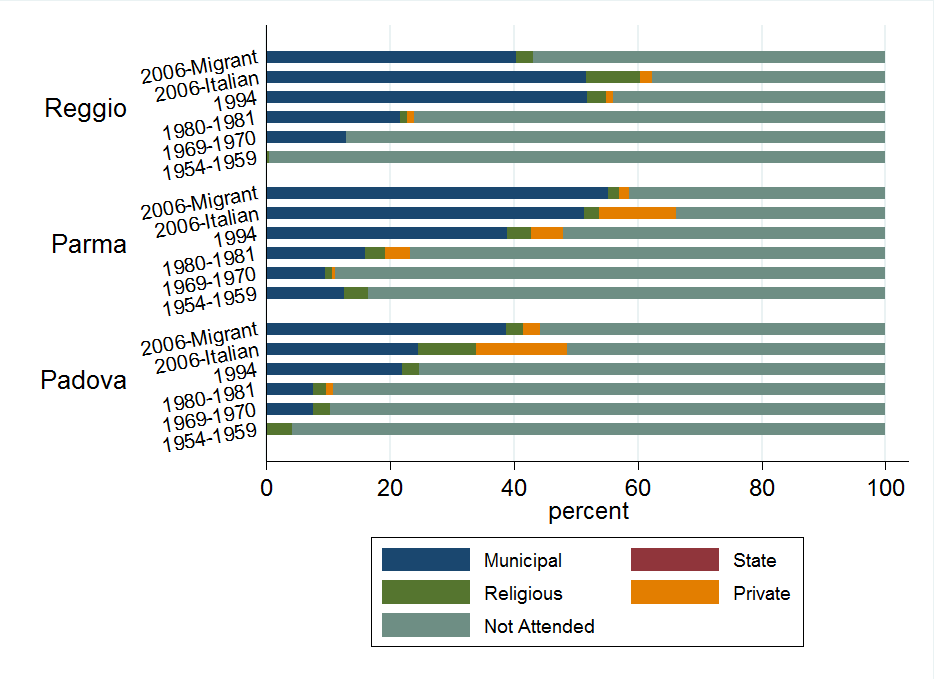
\includegraphics[scale=0.63]{../../../../output/image/asiloType-Attend.png} 
\end{figure}
\end{landscape}


\section{Estimation Strategy} \label{sec:estimation}

Since there are two stages of early childhood interventions, (i) ages 0-3 and (ii) ages 3-6, it is important to consider both when estimating treatment effects of either intervention on later outcomes. Table \ref{tab:cases-treat} shows the possible cases of receiving early childhood intervention in our data, where 0 indicates not attending and 1 indicates attending. For this stage, we limit the type of infant-toddler centers and preschools to municipal only. 

\begin{table}[H] \caption{Possible Cases of Treatment} \label{tab:cases-treat}

  \begin{tabular}{C{1.8cm} R{0.7cm} C{2cm} C{2cm}}
  
		& & \multicolumn{2}{c}{Preschool (Ages 3-6)} \\
		& & 0 & 1 \\ \cline{3-4}            
        								 &  & \multicolumn{1}{|c|}{} & \multicolumn{1}{c|}{} \\
        								& 0 & \multicolumn{1}{|c|}{(0,0)} & \multicolumn{1}{c|}{(0,1)} \\ 
        				ITC				&  & \multicolumn{1}{|c|}{} & \multicolumn{1}{c|}{} \\ \cline{3-4}
                        (Age 0-3)  		&  & \multicolumn{1}{|c|}{} & \multicolumn{1}{c|}{} \\
        								& 1 & \multicolumn{1}{|c|}{(1,0)} & \multicolumn{1}{c|}{(1,1)} \\ 
        								&  & \multicolumn{1}{|c|}{} & \multicolumn{1}{c|}{} \\ \cline{3-4}
  \end{tabular}
\end{table}

There are two main ways of testing treatment effects of attending infant-toddler centers. First is to compare people who did not attend any municipal school for both ages 0-3 and 3-6 with people who only attended municipal infant-toddler centers for ages 0-3. This is to compare (0,0) and (1,0) in Figure \ref{tab:cases-treat}. Second is to compare people who only attended municipal preschool for ages 3-6 with people who attended both municipal infant-toddler centers and preschools. This is to compare (0,1) and (1,1) in Figure \ref{tab:cases-treat}. Formally writing, the hypothesis are:
\begin{eqnarray}
H_1: &  Y_{0,0} = Y_{1,0} \\ 
H_2: &  Y_{0,1} = Y_{1,1} 
\end{eqnarray}
where $Y_{0,0}$ is the outcome of the people who did not attend any infant-toddler center or preschool, and vice versa for other cases. 

\subsection{Strategy 1}

A possible estimation strategy is to limit the sample to specific city \textit{and} specific cohort \textit{and} the comparison groups needed according to the hypothesis above. To test $H_1$, we estimate the following regression equation:
\begin{eqnarray}
Y_{i}^{c,h} & = & \alpha + \beta_{0}R + \mathbf{X}\gamma + \varepsilon_{i}^{c,h}, \\ \nonumber
& \forall & i \in \text{ \{People in city $c$ and cohort $h$ and in group (0,0) or (1,0)\}}
\end{eqnarray}
where $R$ is the indicator for attending municipal infant-toddler center and $\mathbf{X}$ is the vector of baseline variables. Likewise, to test $H_2$:
\begin{eqnarray}
Y_{i}^{c,h} & = & \alpha + \beta_{0}R + \mathbf{X}\gamma + \varepsilon_{i}^{c,h}, \\ \nonumber
& \forall & i \in \text{ \{People in city $c$ and cohort $h$ and in group (0,1) or (1,1)\}}
\end{eqnarray}

One of the caveats of this analysis is that it significantly reduces the sample size used in the analysis. In fact, the hypotheses cannot be tested using this strategy for many groups. Table \ref{tab:num-group} shows the number of people available for each group necessary for analysis using this strategy. It is easy to see that it is impossible to test $H_1$ with our data, because there are almost no people who went to municipal infant-toddler centers but did not attend any preschools (the group (1,0)). It is possible to carry out test for $H_2$ for many groups, but the number of observations for the group (1,1) is very small for the adult cohorts. 

\begin{table}[H] \caption{Number of Individuals in Each Group} \label{tab:num-group}
\scalebox{0.77}{
\begin{tabular}{l|ccccc|ccccc|ccccc}
\toprule
			& 		\multicolumn{5}{c}{\textbf{Reggio}}		& 	\multicolumn{5}{|c|}{\textbf{Parma}}	& 			\multicolumn{5}{c}{\textbf{Padova}}				\\
			& (0,0) & (1,0) & (0,1) & (1,1) & Total & (0,0) & (1,0) & (0,1) & (1,1) & Total  & (0,0) & (1,0) & (0,1) & (1,1) & Total \\ \midrule
Child		& 2 & 0 & 46 & 117 & \textbf{311} & 5 & 1 & 35 & 100 & \textbf{291} & 2 & 0 & 31 & 36 & \textbf{278} \\
Migrant		& 4 & 0	& 24 & 26 & \textbf{110} & 4 & 0 & 12 & 23 & \textbf{58} & 5 & 0 & 18 & 16 & \textbf{113} \\
Adolescent 	& 7 & 0 & 45 &	116 & \textbf{300} & 4 & 0 & 49 & 61 & \textbf{254} & 1 & 0 & 55 & 37 & \textbf{282} \\
Age-30		& 57 & 0 & 95 &	53 & \textbf{280} & 43 & 0 & 64 & 29 & \textbf{251} & 47 & 0 & 25 & 9 & \textbf{251} \\
Age-40		& 80 & 0 & 97 &	28 & \textbf{285} & 115 & 1 & 35 & 16 & \textbf{254} & 75 & 0 & 25 & 2 & \textbf{252} \\
Age-50		& 146 & 0 &	8 & 0 & \textbf{200} & 71 & 0 & 4 & 8 & \textbf{103} & 55 & 0 & 11 & 0 & \textbf{146} \\ \bottomrule
\end{tabular}}
\end{table}

\subsection{Strategy 2}
Another strategy is to use broader sample and control for the preschool attendance in the regression equation. We still divide the groups by city and cohort. We first aim to estimate the effect of attending infant toddler centers in general, $R^{Attend}$, without differentiating among types. That is:
\begin{equation}
Y_{i}^{c,h} = \alpha + \beta_{0}R^{Attend} + \mathbf{P}\delta + \mathbf{X}\gamma + \varepsilon_{i}^{c,h}, \forall i \in \text{ \{People in city $c$ and cohort $h$\}}
\end{equation}
where $\mathbf{P}$ is the vector of indicators of attending each type of preschools for ages 3-6. We then aim to estimate the effect of attending municipal infant-toddler centers by using the following regression equation:
\begin{eqnarray}
Y_{i}^{c,h} & = & \alpha + \beta_{0}R^{None} + \beta_{1}R^{Reli} + \beta_{2}R^{Priv} + \mathbf{P}\delta +  \mathbf{X}\gamma + \varepsilon_{i}^{c,h}, \\ \nonumber
& \forall & i \in \text{ \{People in city $c$ and cohort $h$\}}
\end{eqnarray}

Here, the indicator for attending municipal infant-toddler center is dropped due to collinearity, and this allows the interpretation on the $\beta$ to be the difference in outcome for the corresponding group relative to the people who attended municipal infant-toddler centers. 


\end{document}
